%!TEX root = ../../main.tex
\section{Extending RADDOSE-3D for SAXS}
\label{sec:Extending RADDOSE-3D for SAXS}
To perform comparative analysis of the extent of radiation damage in SAXS experiments it is necessary to calculate the absorbed dose of the sample.
Currently dose estimates in SAXS are calculated using an equation that effectively assumes a 1D model of the experiment (equation 4 in \cite{meisburger2013breaking} and equation 1 in \cite{jeffries2015limiting}).
A more accurate calculation can be performed if the SAXS experiment is simulated in three dimensions providing a spatially resolved dose field.
This dose field can then be interpreted with the various dose metrics already developed for MX \cite{zeldin2013dwd,zeldin2012}.

This section presents the extensions written into RADDOSE-3D to perform simulations of SAXS experiments for improved dose calculations.

\subsection{Cylindrical sample geometry}
\label{sub:Cylindrical sample geometry}
In a typical SAXS experiment, liquid samples are typically flowed through a cylindrical capillary during the X-ray exposure.
Therefore it is necessary for RADDOSE-3D to be able model cylindrical sample shapes.
RADDOSE-3D was extended to handle polygonal shapes \cite{bury2015radiation}, which meant that because any 3D shape can be modelled by a series of polygons, it was already capable of modelling cylindrical shapes.
However the implementation for polyhedral crystals (polyhedra meaning a three dimensional shape composed of a collection of polygons) requires the user to define the sample geometry in a non-user friendly manner.
A file specifying the geometry of the shape by a set of vertex positions and their connectivity is required.
This is much more complex than defining the diameter of the circular cross section and the length/height of a cylinder.
Therefore a module was written that accepts a diameter and height as input and converts this into a polyhedral description (a set of vertices and faces) of a cylinder within RADDOSE-3D.
\begin{figure}
    \centering
    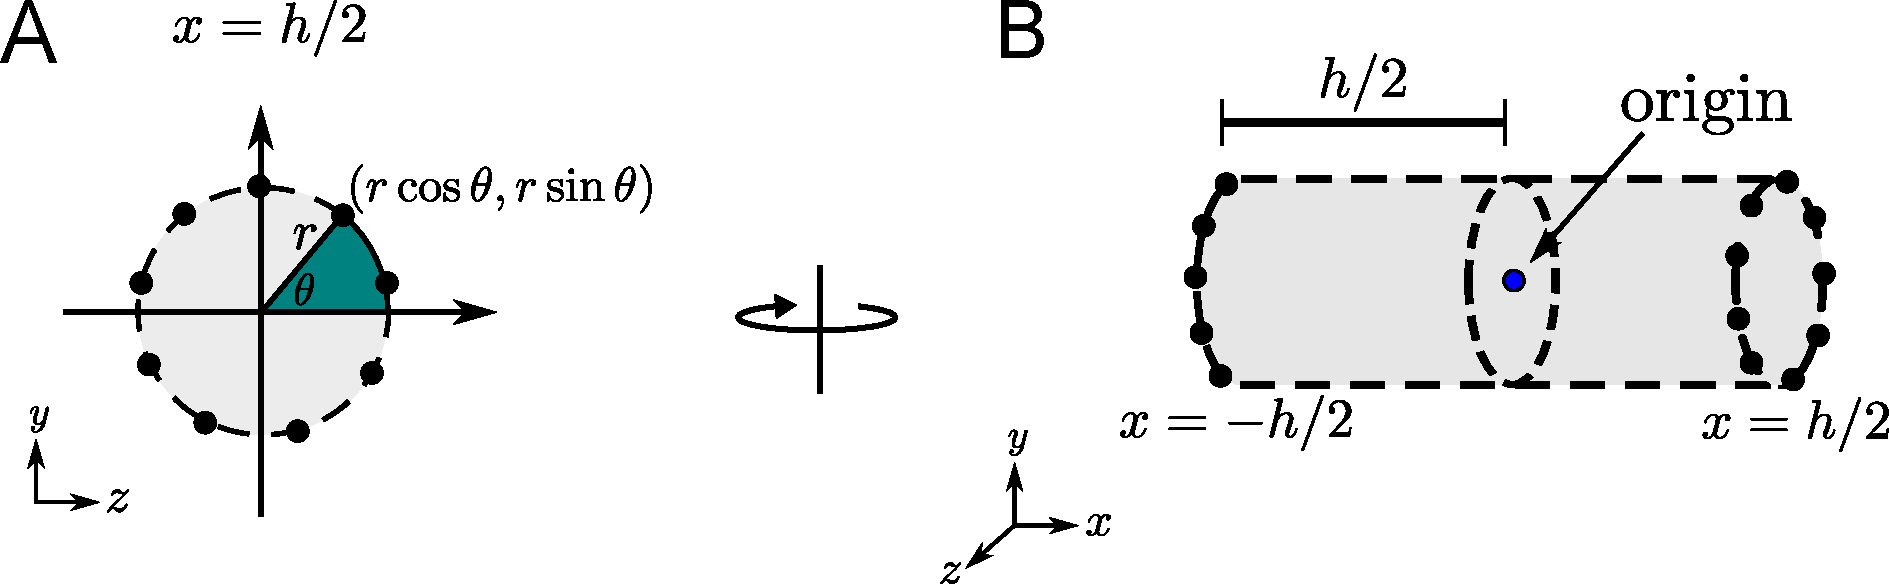
\includegraphics[width=1\textwidth]{figures/saxs/cylinder_implementation.pdf}
    \caption{Implementation of the cylindrical sample geometry in RADDOSE-3D given user defined diameter, $d$ and height $h$. (A) evenly spaced points around a circle are generated given the radius $r = d/2$ of the circular cross-section. RADDOSE-3D defaults to 32 points. (B) In three dimensions the points represent the circles at each end of the cylinder at a distance of $h/2$ from the origin located at the centre of the cylinder. The connectivity of these vertices is hard-coded into the RADDOSE-3D source code.}
    \label{fig:Cylindrical implementation}
\end{figure}

The cylindrical implementation is graphically depicted in Figure~\ref{fig:Cylindrical implementation}.
First the points around a circle are generated using the user defined diameter of the circular cross section.
RADDOSE-3D uses 32 points around the circle by default no matter what dimensions that are specified.
The points are evenly spaced around the circle with $y, z$ coordinates $(r \cos \theta, r \sin \theta)$.
The angle (in radians) between any two consecutive points is $2 \pi / 32$.
A cylinder can be defined by the circles at either end of the shape so this is done using the final coordinate $x$.
Depending on which end a particular point is on it will have coordinates $(x, y, z) = (-h/2, r \cos \theta, r \sin \theta)$ or $(x, y, z) = (h/2, r \cos \theta, r \sin \theta)$.
Note that this assumes the origin of the system is located at the centre of the cylinder.

Regardless of the dimensions of the cylinder, the connectivity of the vertices remains the same because the number of vertices and their orientation with respect to one another is constant.
Therefore the connectivity has been hard-coded into RADDOSE-3D.
It will only ever need to be changed if the number of points is changed.
However this parameter is not exposed to the user and hence it would only change if a developer changed the source code.

The geometry defined to create the cylinder is rotated $90^{\circ}$ about the $y$-axis compared to the RADDOSE-3D simulation geometry.
This means that the beam would irradiate the sample along the $x$-axis (or directly into the page looking at Figure~\ref{fig:Cylindrical implementation} A).
In a typical SAXS experiment the beam direction is along the $z$-axis defined in Figure~\ref{fig:Cylindrical implementation}  (i.e. perpendicular to the axial dimension of the cylinder).
So whenever a user specifies a SAXS experiment in RADDOSE-3D the sample is rotated by an additional $90^{\circ}$ to the angle which the user specifies as the initial orientation of the sample to the beam (the sample geometry does not have to be specified as cylindrical).

The user should also be aware that the dimensions provided in the input file specifies the geometry of the sample alone, not the surrounding capillary. The capillary is dealt with separately (section \ref{sub:Attenuation of X-ray flux due to capillary})

\subsection{Determining the sample composition}
\label{sub:Determining the sample composition}
Knowledge of the atomic composition of the sample is necessary to be able to calculate the absorbed dose upon X-ray irradiation.
This is because the overall absorption coefficient of the sample is calculated from the individual atomic absorption coefficients \cite{murray2004}.
In MX the crystal composition is calculated from the contents of the unit cell.
In SAXS the samples are liquids as opposed to crystals and hence the notion of a unit cell does not apply.
So instead the approach to determine the atomic composition of the sample is to define a volume of liquid and estimate its contents given the protein concentration and buffer composition of the liquid solution.

First the molarity of the solution is calculated using the formula
\begin{equation}
    \text{Molarity (moles/litre)} = \f{\text{sample concentration (grams/litre)}}{\text{molecular mass (grams/mole)}}.
    \label{eq:molarity calculation}
\end{equation}
The sample concentration is provided by the user in units of grams per litre.
The molecular mass of the molecule is calculated from other parameters provided in the user input.
If the sequence file is given for the protein (the sample could also contain DNA and RNA) then the molecular mass can be determined accurately by summing the molecular mass of each residue in the file.
Otherwise an average molecular weight is used for each residue (110 daltons for protein residues, 339.5 daltons for RNA residues and 327 daltons for DNA residues) and the user has to specify the type and number of residues for the sample.

Secondly a suitable volume needs to be specified to calculate the atomic composition.
A suitable volume is one that is large enough to contain at least one complete molecule.
By default this volume is defined to be $1 \times 10^9$\AA$^3$ but this can be changed by specifying the length, width and height dimensions of the volume in the input file using the \textit{unit cell} input keyword.

The number of monomers/molecules in the volume can now be calculated by multiplying the molarity, volume (converted to litres) and Avogadro's number ($N_A = 6.022 \times 10^{23} mol^{-1}$), which is then rounded to the nearest integer.
The absorption coefficient can then be calculated in the usual way as is described in \cite{pait2009}.
If there is less than 1 molecule in the volume then this is flagged up and the user is advised to increase the volume.

\subsection{Attenuation of X-ray flux due to capillary}
\label{sub:Attenuation of X-ray flux due to capillary}
In a typical MX experiment a crystal is exposed directly to the X-ray beam.
In contrast, samples from SAXS experiments are held inside a capillary.
This means that the attenuation of the X-ray flux due to the capillary needs to be taken into account before calculating the absorbed dose in the sample.

The transmission fraction of an X-ray beam due to a material with mass thickness $x$ and density $\rho$ is given by
\begin{equation}
    I/I_0 = \exp \left[ -(\mu/\rho)x\right],
    \label{eq:capillary transmission fraction}
\end{equation}
where $I$ is the emergent intensity of the beam after penetrating the material, $I_0$ is the incident intensity and $\mu/\rho$ is defined as the mass attenuation coefficient \cite{hubbell1995tables}.
The mass thickness, $x$, is defined as the mass per unit area and is given by $x = \rho t$ where $t$ is the thickness of the material.
The attenuation fraction by the capillary can hence be calculated as $1 - I/I_0$.

RADDOSE-3D requires the user to supply the thickness, density and material composition of the capillary to calculate the attenuation fraction.
The mass thickness can be directly calculated using the density and thickness as described above.
The mass attenuation coefficient is dependent on the atomic composition of the material as well as the energy of the incident photons.
The relevant values can be found online via the National Institute of Science and Technology (NIST) tables \cite{nisttable3,nisttable4}.
A section of the webpage for the mass attenuation coefficient table of carbon is shown in Figure~\ref{fig:NIST table for carbon}.
\begin{figure}
    \centering
    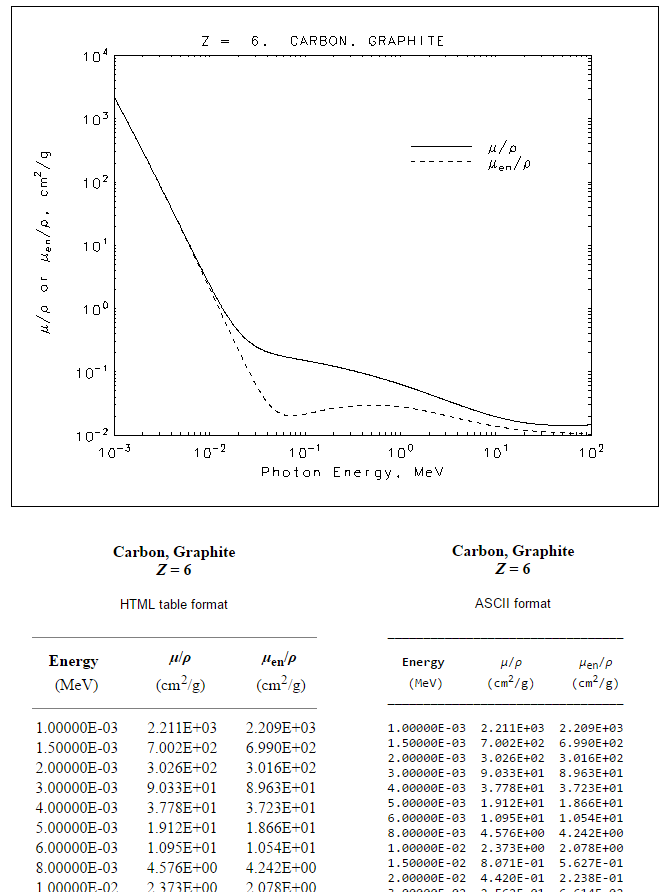
\includegraphics[width=0.8\textwidth]{figures/saxs/nist_table_carbon.png}
    \caption{Section of the X-ray mass attenuation coefficient data for carbon. The mass attenuation coefficient data are tabulated beneath the graph. The exact energy of the X-ray photons used in crystallography and SAXS (typically around $12\ keV$) is explicitly tabulated therefore the mass attenuation coefficient is obtained by linear interpolation.}
    \label{fig:NIST table for carbon}
\end{figure}
The tabulated energy values do not explicitly include the typycial energies used in crystallograpy and SAXS (around $12\ keV$), so the mass attenuation coefficient is linearly interpolated between the closest values.
Mass attenuation coefficient data for various mixtures including air, borosilicate glass, water, bone and soft tissue are also tabulated in NIST table 4 \cite{nisttable4}.
These mixtures can be used directly by RADDOSE-3D.

When mixtures of atomic species are used (the most commonly used capillary material in SAXS is quartz which has elemental composition $SiO_2$) the mass attenuation coefficient is obtained using a weighted average given by
\begin{equation}
    \mu/\rho = \sum_i w_i (\mu/\rho)_i,
\end{equation}
where $w_i$ and $(\mu/\rho)_i$ are the fraction by weight and mass attenuation coefficient of the $i^{\text{th}}$ atomic constituent respectively.

\subsection{Model considerations}
\label{sub:Model considerations}
The model of the SAXS experiment in RADDOSE-3D makes many implicit assumptions.
With regards to the capillary, the atomic composition is uniform throughout and the thickness is assumed constant around the entire sample volume.
The advantage of this assumption is that the attenuation by the capillary only needs to be calculated once regardless of any movement or rotation of the capillary.
These assumptions are valid for a cylindrical capillary since the thickness penetrated by the X-ray beam is the same regardless of any rotations or translations.

The sample itself is assumed static, moves as a rigid body and completely fills the capillary.
This greatly reduces the computational cost when compared to the possibility of modelling the exact fluid dynamics.
The assumption that the capillary volume is completely filled is valid for most cases since this is usually the case during an experiment.
The static assumption is not always valid, especially when the sample is flowed through the capillary.
However the rigid body assumption may still hold.
During the time that the sample is flowed through the X-ray beam, a small volume element of water may have a constant position with respect to another small volume element of fluid.
In other words, the fluid sample moves as one rigid body in the time it takes to pass through the X-ray beam.
To verify this assumption SAXS experiments would have to be performed where the damage rates and signatures are found in runs where the fluid is kept static.
Then those results would have to be compared to results obtained from experiments where the sample is flowed through the capillary, and doses are calculated using the rigid body assumption to observe whether similar damage rates and signatures are observed.

The SAXS sample can also be manipulated in the same way as a crystal in RADDOSE-3D.
Hence helical scanning, translations and rotations of the sample can all be performed.
Figure~\ref{fig:SAXS cylinder rotated} is the final dose state of a glucose isomerase sample in an experiment where the sample was rotated $180^{\circ}$ in a $ 700 \mu m \times 700 \mu m $ top-hat profile beam.
\begin{figure}
    \centering
    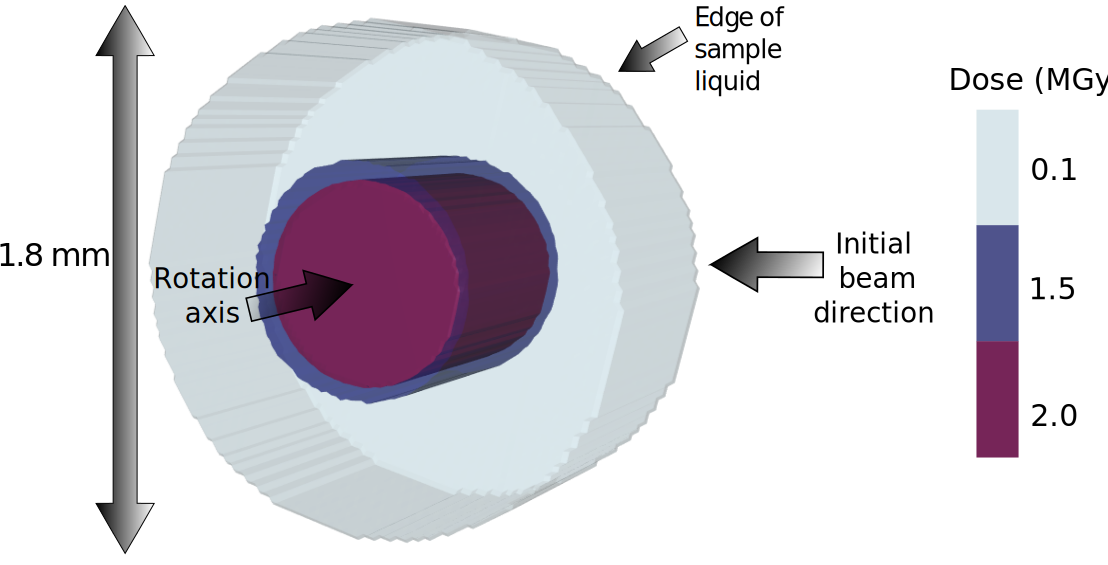
\includegraphics[width=0.5\textwidth]{figures/saxs/SAXScylinder.png}
    \caption{Final dose state of a glucose isomerase sample in an experiment where the sample was rotated $180^{\circ}$ in a $ 700 \mu m \times 700 \mu m $ top-hat profile beam with an incident energy of $ 12.1 keV $ for a total exposure time of 200 seconds. The capillary was treated as completely transparent to the X-rays so there was no attenuation. The contours correspond to dose iso-surfaces: light blue = $ 0.1\ MGy $, dark blue = $ 1.5\ MGy $ and red = $ 2\ MGy $ }
    \label{fig:SAXS cylinder rotated}
\end{figure}
